
\label{cap_conclusoes}

em trabs futuros:

tentar provar analiticamente a conjectura para arvores lineares

testar renomeamentos com limite de subformulas (seria mt bom, pq os provers sao exponenciais justamente no nro de simbolos proposicionais. fazer dois graficos com crescimentos opostos pra ilustrar esse problema. além disso, quanto menor for o tamanho maximo do renomeamento, mais próxima a complexidade do knapsack fica da complexidade do Boy dela tour!)

adaptar o algoritmo para outras formas normais e/ou outras metricas de minimizacao

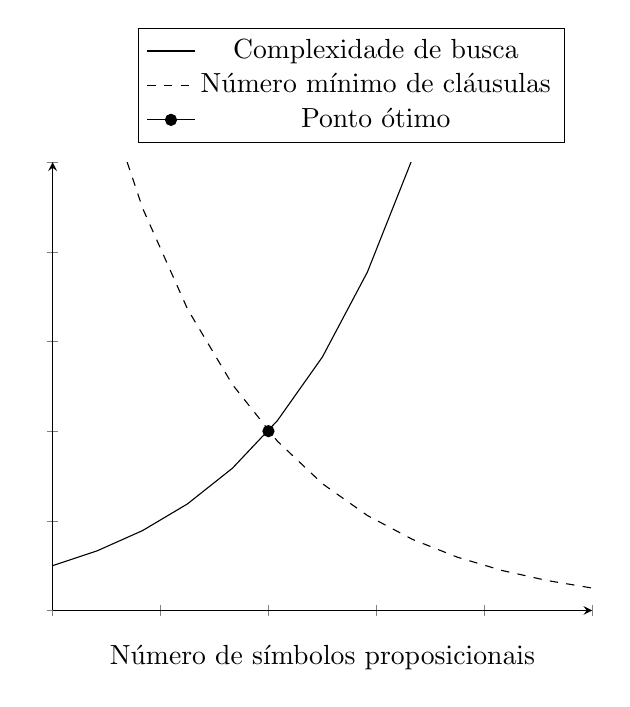
\begin{tikzpicture}
\begin{axis}[ymin=0,ymax=10,xmin=0,xlabel=Número de símbolos proposicionais,yticklabels={,,},xticklabels={,,},axis lines = left,legend entries={Complexidade de busca,Número mínimo de cláusulas,Ponto ótimo},legend style={at={(.95,1.3)}}]
\addplot[mark=none]{2^x};
\addplot[mark=none,dashed]{2^(4-x)};
\addplot[mark=*] coordinates {(2,4)};;
\end{axis}
\end{tikzpicture}